\subsection{カードリスト画面}
カードリスト画面とは、木古内で「できること」に着目した観光情報を写真と紹介文でリストにしてカードのように表示する画面のことを言う。一枚のカードに含まれる情報は、そのスポットの写真、キャッチコピーの様なタイトル、紹介文、そして4つのボタンである。ボタンについては表6.1を参照されたい。そしてアプリの画面を図6.1で紹介する。ユーザはキーコ紀行をダウンロードしたらまずこの画面を見て、気になったらそのスポットへ向かう、といったユーザストーリ―を想定している。使用されている写真は、実際に我々が木古内に行き、撮影したものを使用している。タイトルや紹介文は、メンバーで考えた約70字という制限がついた文である。この画面からは、マップ・詳細画面、写真撮影画面、テキスト編集画面に遷移できる。

\begin{table}[htb]
\centering
\addtocounter{table}{+0}
\caption{カードリストのボタンのアイコンとその意味}
  \begin{tabular}{|c|c|} \hline
    アイコン&意味  \\ \hline 
    \begin{minipage}{10mm}
      \centering
      \scalebox{0.4}{
\includegraphics{pencil.png}}
    \end{minipage} & \parbox{38zw}{テキストを編集画面へ遷移するボタン。} \\  \hline
    \begin{minipage}{10mm}
      \centering
      \scalebox{0.4}{
\includegraphics{pin.png}}
    \end{minipage} &\parbox{38zw}{マップ・詳細画面へ遷移するボタン。}\\ \hline
     \begin{minipage}{10mm}
      \centering
      \scalebox{0.4}{
\includegraphics{camera.png}}
    \end{minipage} & \parbox{38zw}{写真撮影画面へ遷移するボタン。}\\ \hline
	\begin{minipage}{10mm}
      \centering
      \scalebox{0.4}{
\includegraphics{favourites_glay.png}}
    \end{minipage} & \parbox{38zw}{いわゆる「ブックマーク」のようなボタン。ユーザが気に入ったらこのボタンを押し、マップ詳細画面で違うスポットを見たときにでも場所がわかるようになる。} \\  \hline
  \end{tabular} 
\end{table}

\begin{figure}[htbp]
 \begin{center}
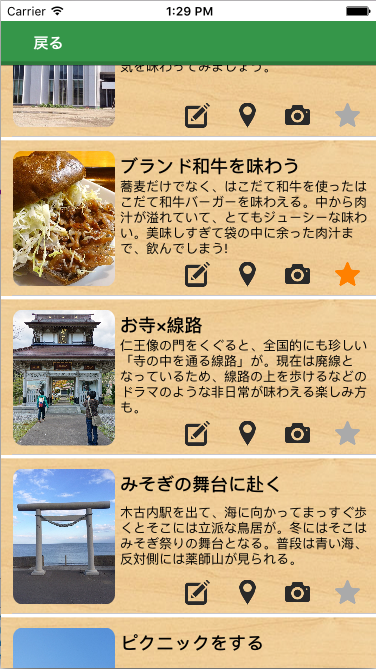
\includegraphics[width=4cm, bb=0 0 303 573]{cardList.png}
 \end{center}
\addtocounter{figure}{+0}
 \caption{カードリスト画面}
 \label{fig:one}
\end{figure}

\bunseki{山川拓也}